\documentclass[12pt]{article}

\usepackage[english]{babel}
\usepackage[utf8]{inputenc}
\usepackage[top=0.5cm, left=0.5cm, right=0.5cm, bottom=2cm]{geometry}
\usepackage[document]{ragged2e}
\usepackage{tikz,minted,times}

\setlength\parindent{0pt}
\sloppy
\usetikzlibrary{automata,positioning,arrows,fit}
\tikzset{node distance=2.5cm,every state/.style={semithick,fill=gray!10},initial text={},double distance=2pt,every edge/.style={draw,->,>=stealth,auto,semithick}}
\usemintedstyle{colorful}

\title{COMP SCI 7411 Event Driven Computing Practice 3 Plan}
\author{Tinson Lai \\ a1812422}
\date{}

\begin{document}

\maketitle

Due to the constraint that train will not change direction, the following routes are the only options for trains entering the system.

\begin{itemize}
  \item Train entering from $1$ going east

    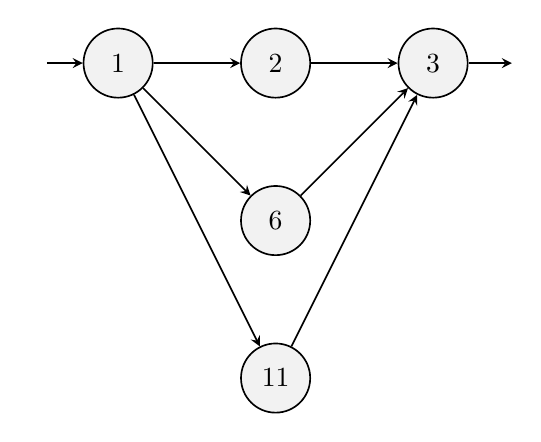
\begin{tikzpicture}
      \node[state, initial] at (0, 4) (1){1};
      \node[state] at (2, 4) (2){2};
      \node[state] at (2, 2) (6){6};
      \node[state] at (2, 0) (11){11};
      \node[state] at (4, 4) (3){3};

      \draw

      (1) edge (2)
      (1) edge (6)
      (1) edge (11)

      (2) edge (3)
      (6) edge (3)
      (11) edge (3)

      (3) edge +(1, 0)

      ;
    \end{tikzpicture}
  \item Train entering from $4$ going east

    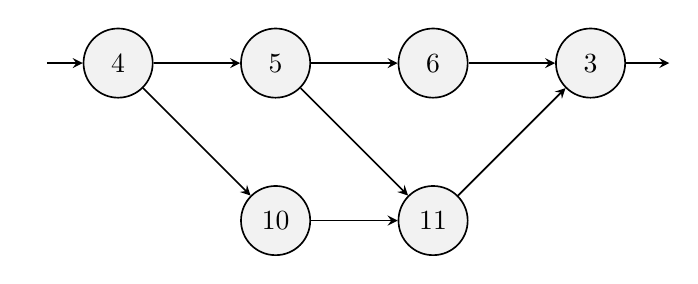
\begin{tikzpicture}
      \node[state, initial] at (0, 2) (4){4};
      \node[state] at (2, 2) (5){5};
      \node[state] at (4, 2) (6){6};
      \node[state] at (6, 2) (3){3};
      \node[state] at (2, 0) (10){10};
      \node[state] at (4, 0) (11){11};

      \draw

      (4) edge (5)
      (4) edge (10)

      (5) edge (6)
      (5) edge (11)
      (10) edge (11)

      (6) edge (3)
      (11) edge (3)

      (3) edge +(1, 0)

      ;
    \end{tikzpicture}
  \item Train entering from $8$ going west

    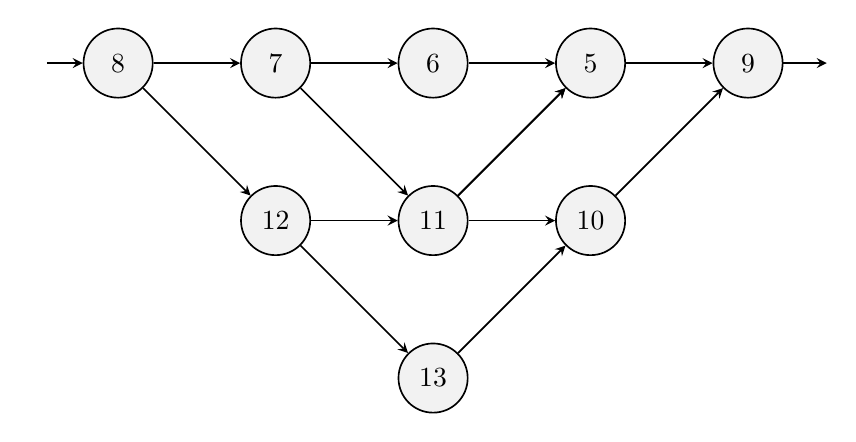
\begin{tikzpicture}
      \node[state, initial] at (0, 4) (8){8};
      \node[state] at (2, 4) (7){7};
      \node[state] at (4, 4) (6){6};
      \node[state] at (6, 4) (5){5};
      \node[state] at (8, 4) (9){9};
      \node[state] at (2, 2) (12){12};
      \node[state] at (4, 2) (11){11};
      \node[state] at (6, 2) (10){10};
      \node[state] at (4, 0) (13){13};

      \draw

      (8) edge (7)
      (8) edge (12)

      (7) edge (6)
      (7) edge (11)

      (12) edge (11)
      (12) edge (13)

      (11) edge (5)
      (11) edge (10)

      (13) edge (10)

      (6) edge (5)
      (11) edge (5)

      (5) edge (9)
      (10) edge (9)

      (9) edge +(1, 0)

      ;
    \end{tikzpicture}
\end{itemize}

In the following sections, I will use the following notations in the Petri Net, where in the Petri Net tuple $N=\left(P,T,A,W,I\right)$

\begin{itemize}
  \item ($P$) $p_i$ refers to track $i$ when it's empty. $p_{i,e}$ or $p_{i,w}$ refers to track $i$ with a east direction ($e$) or west direction ($w$) train on it. This is a necessary notation to avoid deadlock.  All $p_i$ with $p_{i,e}$ and $p_{i,w}$ forms different buffers in the Petri Net.
  \item ($P$) $d_i$ refers to a dispatcher, where only $d_1$, $d_4$ and $d_8$ are available as trains can only enter the system from these tracks. They also act as producers in the Petri Net as well.
  \item ($P$) $o_i$ refers to the outgoing track, where only $o_3$ and $o_9$ are available as trains can only exit the system from these tracks. They also act as consumers in the Petri Net as well.
  \item ($T$) ${add_i}$ and ${out_i}$ means adding/removing a train from the inbound/outbound track.
  \item ($T$) $m_{i,j}$ refers to a move from track $i$ to track $j$ in train's own direction.
  \item ($T$) $m_{i,j}\left({p_{cond}}\right)$ means a movement is based on a condition of a track, where $p_{cond}$ should also be a state in the Petri Net. It is used to distinguished transition based on a precondition to avoid deadlock in the Petri Net.
  \item $W$ will always be one for all transitions.
  \item ($I$) All $p_i$, $d_i$ and $o_i$ will be an initial states as implied by the definition of producer, consumer and buffer. It is also obvious that the initial system will be completely empty, so the initial state should be neither $p_{i,e}$ nor $p_{1,w}$ but $p_i$.
\end{itemize}

\section{Entering from $1$}

There will be no chance of deadlock in any routes available for train entering from 1, as the intermediate tracks $2$, $6$ and $11$ can reach track $3$ directly so trains in this part can safely pass through any intersections involved in this part.. The only requirement for the move is that the destination track needs to be empty.

\subsection{$1 \rightarrow 2 \rightarrow 3$}

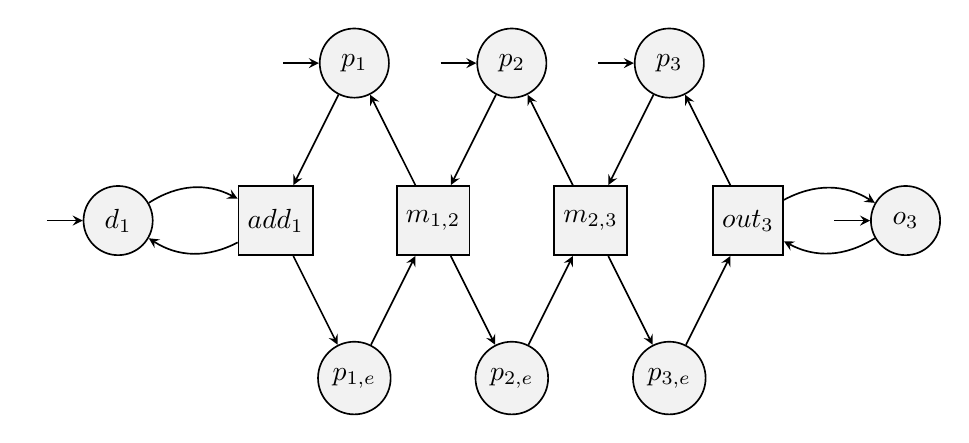
\begin{tikzpicture}
  \node[state, initial] at (0, 2) (d1){$d_1$};
  \node[state, initial] at (10, 2) (o3){$o_3$};

  \node[state, initial] at (3, 4) (p1){$p_1$};
  \node[state, initial] at (5, 4) (p2){$p_2$};
  \node[state, initial] at (7, 4) (p3){$p_3$};

  \node[state] at (3, 0) (p1_e){$p_{1,e}$};
  \node[state] at (5, 0) (p2_e){$p_{2,e}$};
  \node[state] at (7, 0) (p3_e){$p_{3,e}$};

  \node[state, rectangle] at (2, 2) (add1){${add}_1$};
  \node[state, rectangle] at (4, 2) (m1_2){$m_{1,2}$};
  \node[state, rectangle] at (6, 2) (m2_3){$m_{2,3}$};
  \node[state, rectangle] at (8, 2) (out3){${out}_3$};

  \draw

  (d1) edge[bend left] (add1)
  (add1) edge[bend left] (d1)
  (p1) edge (add1)
  (add1) edge (p1_e)

  (p1_e) edge (m1_2)
  (m1_2) edge (p1)
  (p2) edge (m1_2)
  (m1_2) edge (p2_e)

  (p2_e) edge (m2_3)
  (m2_3) edge (p2)
  (p3) edge (m2_3)
  (m2_3) edge (p3_e)

  (p3_e) edge (out3)
  (out3) edge (p3)
  (o3) edge[bend left] (out3)
  (out3) edge[bend left] (o3)

  ;
\end{tikzpicture}

\subsection{$1 \rightarrow 6 \rightarrow 3$}

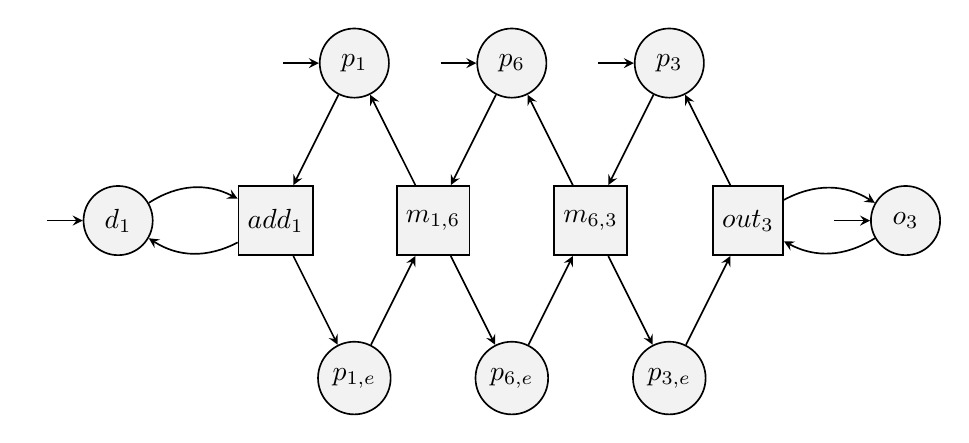
\begin{tikzpicture}
  \node[state, initial] at (0, 2) (d1){$d_1$};
  \node[state, initial] at (10, 2) (o3){$o_3$};

  \node[state, initial] at (3, 4) (p1){$p_1$};
  \node[state, initial] at (5, 4) (p6){$p_6$};
  \node[state, initial] at (7, 4) (p3){$p_3$};

  \node[state] at (3, 0) (p1_e){$p_{1,e}$};
  \node[state] at (5, 0) (p6_e){$p_{6,e}$};
  \node[state] at (7, 0) (p3_e){$p_{3,e}$};

  \node[state, rectangle] at (2, 2) (add1){${add}_1$};
  \node[state, rectangle] at (4, 2) (m1_6){$m_{1,6}$};
  \node[state, rectangle] at (6, 2) (m6_3){$m_{6,3}$};
  \node[state, rectangle] at (8, 2) (out3){${out}_3$};

  \draw

  (d1) edge[bend left] (add1)
  (add1) edge[bend left] (d1)
  (p1) edge (add1)
  (add1) edge (p1_e)

  (p1_e) edge (m1_6)
  (m1_6) edge (p1)
  (p6) edge (m1_6)
  (m1_6) edge (p6_e)

  (p6_e) edge (m6_3)
  (m6_3) edge (p6)
  (p3) edge (m6_3)
  (m6_3) edge (p3_e)


  (p3_e) edge (out3)
  (out3) edge (p3)
  (o3) edge[bend left] (out3)
  (out3) edge[bend left] (o3)

  ;
\end{tikzpicture}

\subsection{$1 \rightarrow 11 \rightarrow 3$}

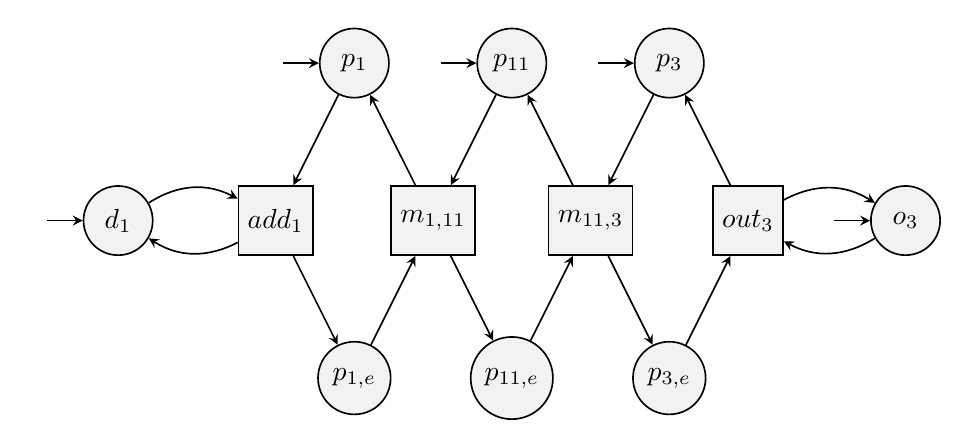
\begin{tikzpicture}
  \node[state, initial] at (0, 2) (d1){$d_1$};
  \node[state, initial] at (10, 2) (o3){$o_3$};

  \node[state, initial] at (3, 4) (p1){$p_1$};
  \node[state, initial] at (5, 4) (p11){$p_{11}$};
  \node[state, initial] at (7, 4) (p3){$p_3$};

  \node[state] at (3, 0) (p1_e){$p_{1,e}$};
  \node[state] at (5, 0) (p11_e){$p_{11,e}$};
  \node[state] at (7, 0) (p3_e){$p_{3,e}$};

  \node[state, rectangle] at (2, 2) (add1){${add}_1$};
  \node[state, rectangle] at (4, 2) (m1_11){$m_{1,11}$};
  \node[state, rectangle] at (6, 2) (m11_3){$m_{11,3}$};
  \node[state, rectangle] at (8, 2) (out3){${out}_3$};

  \draw

  (d1) edge[bend left] (add1)
  (add1) edge[bend left] (d1)
  (p1) edge (add1)
  (add1) edge (p1_e)

  (p1_e) edge (m1_11)
  (m1_11) edge (p1)
  (p11) edge (m1_11)
  (m1_11) edge (p11_e)

  (p11_e) edge (m11_3)
  (m11_3) edge (p11)
  (p3) edge (m11_3)
  (m11_3) edge (p3_e)


  (p3_e) edge (out3)
  (out3) edge (p3)
  (o3) edge[bend left] (out3)
  (out3) edge[bend left] (o3)

  ;
\end{tikzpicture}

\section{Entering from $4$}

Unlike trains coming from $1$, it is possible for trains coming from $4$ and $8$ to entre a deadlock situation when $5$ and $10$ both have a train driving east but both $6$ and $11$ have a train driving west. It is important to ensure that one of the tracks is empty, or at least, one of the tracks having a train travelling in a correct direction which can escape from the congestion.

\subsection{$4 \rightarrow 5 \rightarrow 6 \rightarrow 3$}

To avoid deadlock, $m_{4,5}$ should happen only if one of the following mappings are a subset of the current marking of the Petri Net

\begin{itemize}
  \item $\left\{ p_6 \rightarrow 1 \right\}$
  \item $\left\{ p_{6,e} \rightarrow 1 \right\}$
  \item $\left\{ p_{11} \rightarrow 1 \right\}$
  \item $\left\{ p_{11,e} \rightarrow 1 \right\}$
  \item $\left\{ p_{10} \rightarrow 1 \right\}$
  \item $\left\{ p_{10,w} \rightarrow 1 \right\}$
\end{itemize}

Then the graph for this route will be

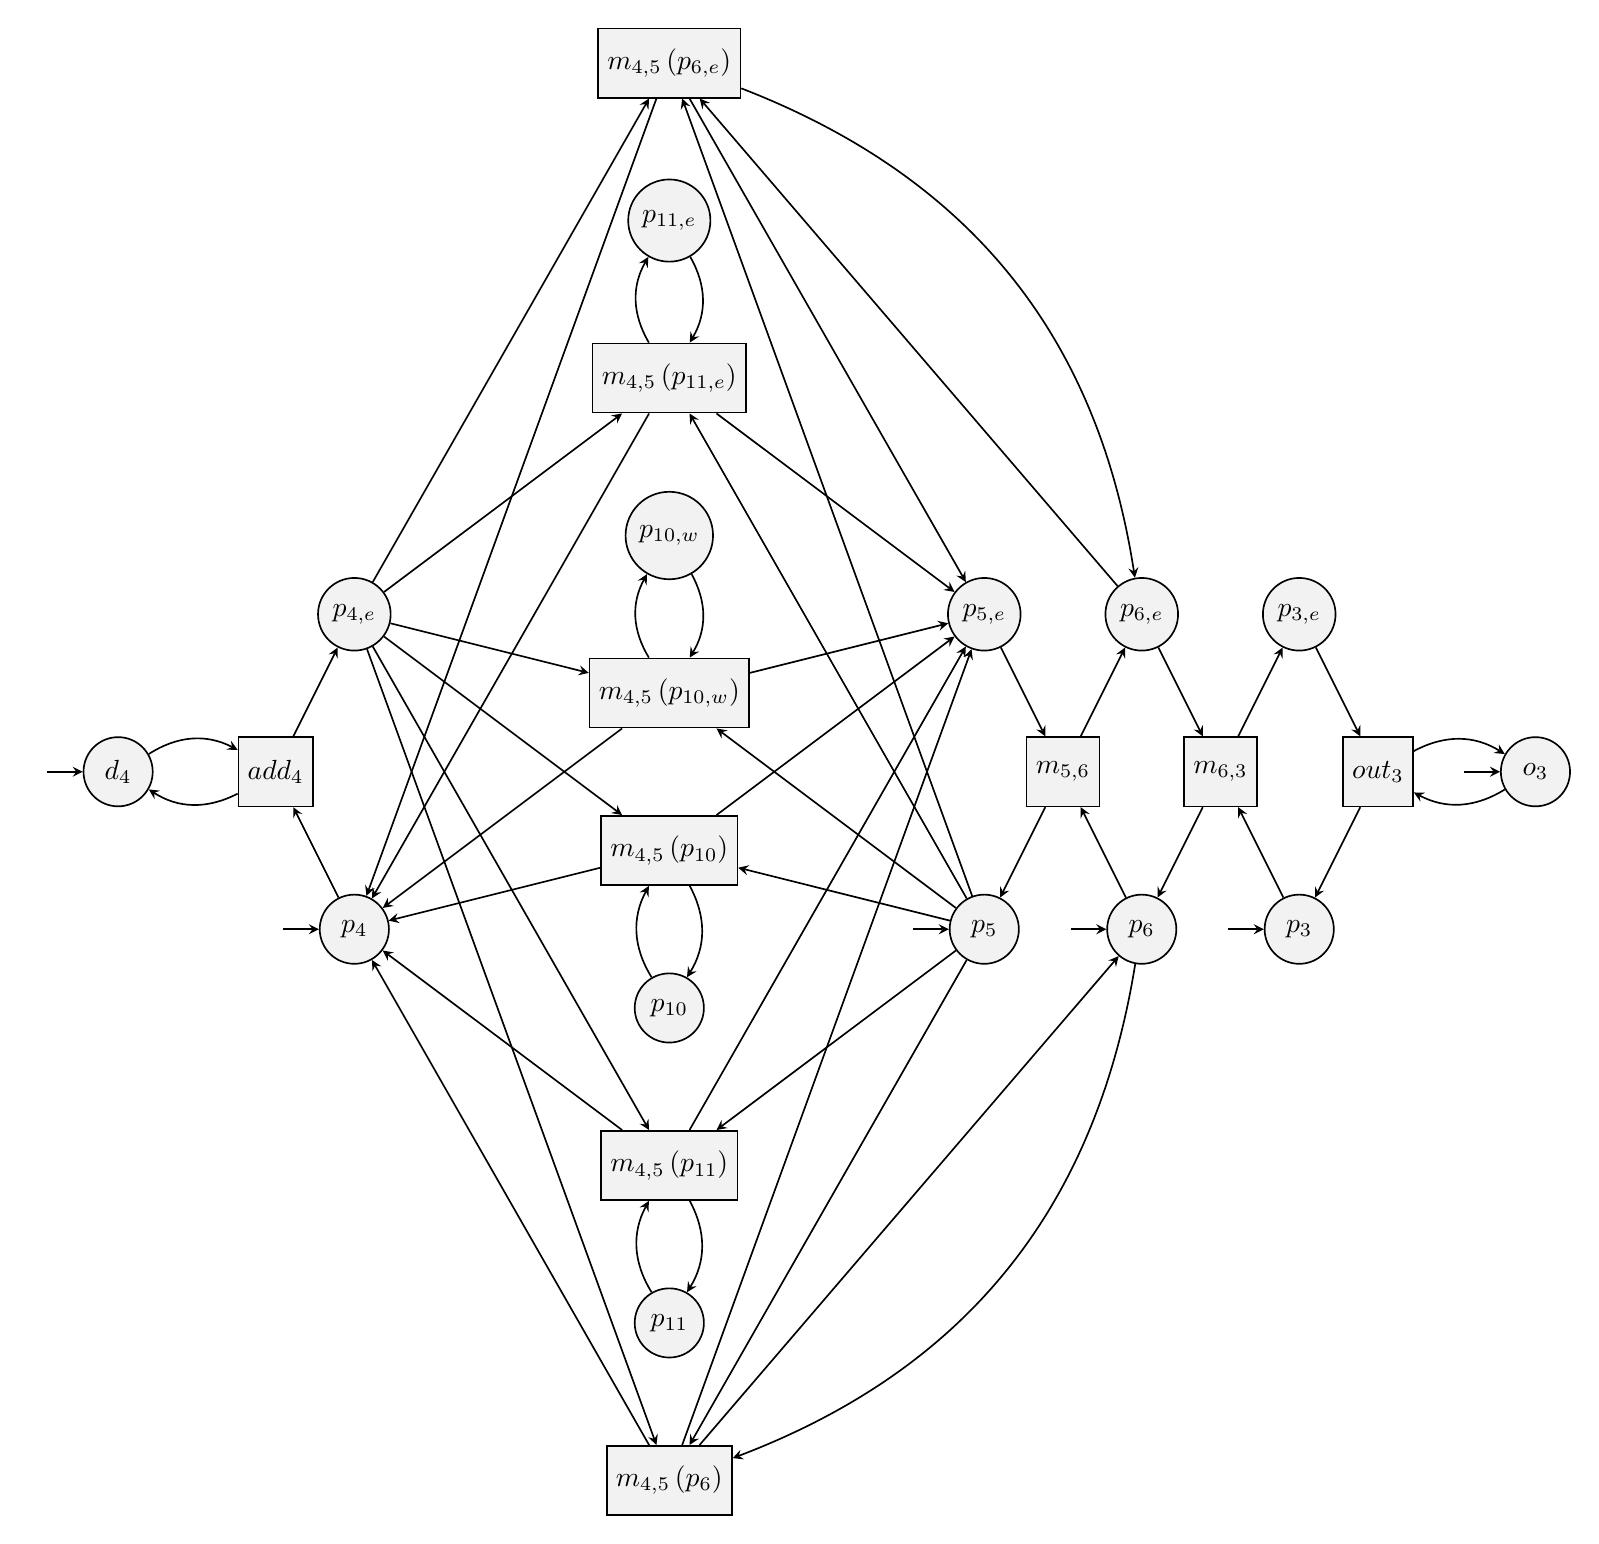
\begin{tikzpicture}
  \node[state, initial] at (0, 11) (d4){$d_4$};
  \node[state, initial] at (18, 11) (o3){$o_3$};

  \node[state, initial] at (3, 9) (p4){$p_4$};
  \node[state, initial] at (11, 9) (p5){$p_5$};
  \node[state, initial] at (13, 9) (p6){$p_6$};
  \node[state, initial] at (15, 9) (p3){$p_3$};

  \node[state] at (3, 13) (p4_e){$p_{4,e}$};
  \node[state] at (11, 13) (p5_e){$p_{5,e}$};
  \node[state] at (13, 13) (p6_e){$p_{6,e}$};
  \node[state] at (15, 13) (p3_e){$p_{3,e}$};

  \node[state, rectangle] at (2, 11) (add4){${add}_4$};
  \node[state, rectangle] at (12, 11) (m5_6){$m_{5,6}$};
  \node[state, rectangle] at (14, 11) (m6_3){$m_{6,3}$};
  \node[state, rectangle] at (16, 11) (out3){${out}_3$};

  \node[state] at (7, 4) (p11){$p_{11}$};
  \node[state] at (7, 8) (p10){$p_{10}$};
  \node[state] at (7, 18) (p11_e){$p_{11,e}$};
  \node[state] at (7, 14) (p10_w){$p_{10,w}$};

  \node[state, rectangle] at (7, 2) (m4_5__p6){$m_{4,5}\left(p_6\right)$};
  \node[state, rectangle] at (7, 6) (m4_5__p11){$m_{4,5}\left(p_{11}\right)$};
  \node[state, rectangle] at (7, 10) (m4_5__p10){$m_{4,5}\left(p_{10}\right)$};
  \node[state, rectangle] at (7, 20) (m4_5__p6_e){$m_{4,5}\left(p_{6,e}\right)$};
  \node[state, rectangle] at (7, 16) (m4_5__p11_e){$m_{4,5}\left(p_{11,e}\right)$};
  \node[state, rectangle] at (7, 12) (m4_5__p10_w){$m_{4,5}\left(p_{10,w}\right)$};

  \draw

  (d4) edge[bend left] (add4)
  (add4) edge[bend left] (d4)
  (p4) edge (add4)
  (add4) edge (p4_e)

  (p4_e) edge (m4_5__p6)
  (p4_e) edge (m4_5__p11)
  (p4_e) edge (m4_5__p10)
  (p4_e) edge (m4_5__p6_e)
  (p4_e) edge (m4_5__p11_e)
  (p4_e) edge (m4_5__p10_w)

  (m4_5__p6) edge (p4)
  (m4_5__p11) edge (p4)
  (m4_5__p10) edge (p4)
  (m4_5__p6_e) edge (p4)
  (m4_5__p11_e) edge (p4)
  (m4_5__p10_w) edge (p4)

  (p5) edge (m4_5__p6)
  (p5) edge (m4_5__p11)
  (p5) edge (m4_5__p10)
  (p5) edge (m4_5__p6_e)
  (p5) edge (m4_5__p11_e)
  (p5) edge (m4_5__p10_w)

  (m4_5__p6) edge (p5_e)
  (m4_5__p11) edge (p5_e)
  (m4_5__p10) edge (p5_e)
  (m4_5__p6_e) edge (p5_e)
  (m4_5__p11_e) edge (p5_e)
  (m4_5__p10_w) edge (p5_e)

  (p5_e) edge (m5_6)
  (m5_6) edge (p5)
  (p6) edge (m5_6)
  (m5_6) edge (p6_e)

  (p6_e) edge (m6_3)
  (m6_3) edge (p6)
  (p3) edge (m6_3)
  (m6_3) edge (p3_e)

  (p3_e) edge (out3)
  (out3) edge (p3)
  (o3) edge[bend left] (out3)
  (out3) edge[bend left] (o3)

  (p6) edge[bend left] (m4_5__p6)
  (m4_5__p6) edge (p6)
  (p6_e) edge (m4_5__p6_e)
  (m4_5__p6_e) edge[bend left] (p6_e)

  (p11) edge[bend left] (m4_5__p11)
  (m4_5__p11) edge[bend left] (p11)
  (p10) edge[bend left] (m4_5__p10)
  (m4_5__p10) edge[bend left] (p10)

  (p11_e) edge[bend left] (m4_5__p11_e)
  (m4_5__p11_e) edge[bend left] (p11_e)
  (p10_w) edge[bend left] (m4_5__p10_w)
  (m4_5__p10_w) edge[bend left] (p10_w)

  ;
\end{tikzpicture}

\subsection{$4 \rightarrow 5 \rightarrow 11 \rightarrow 3$}

The condition is the same as the previous route, but the graph needs to be rearranged

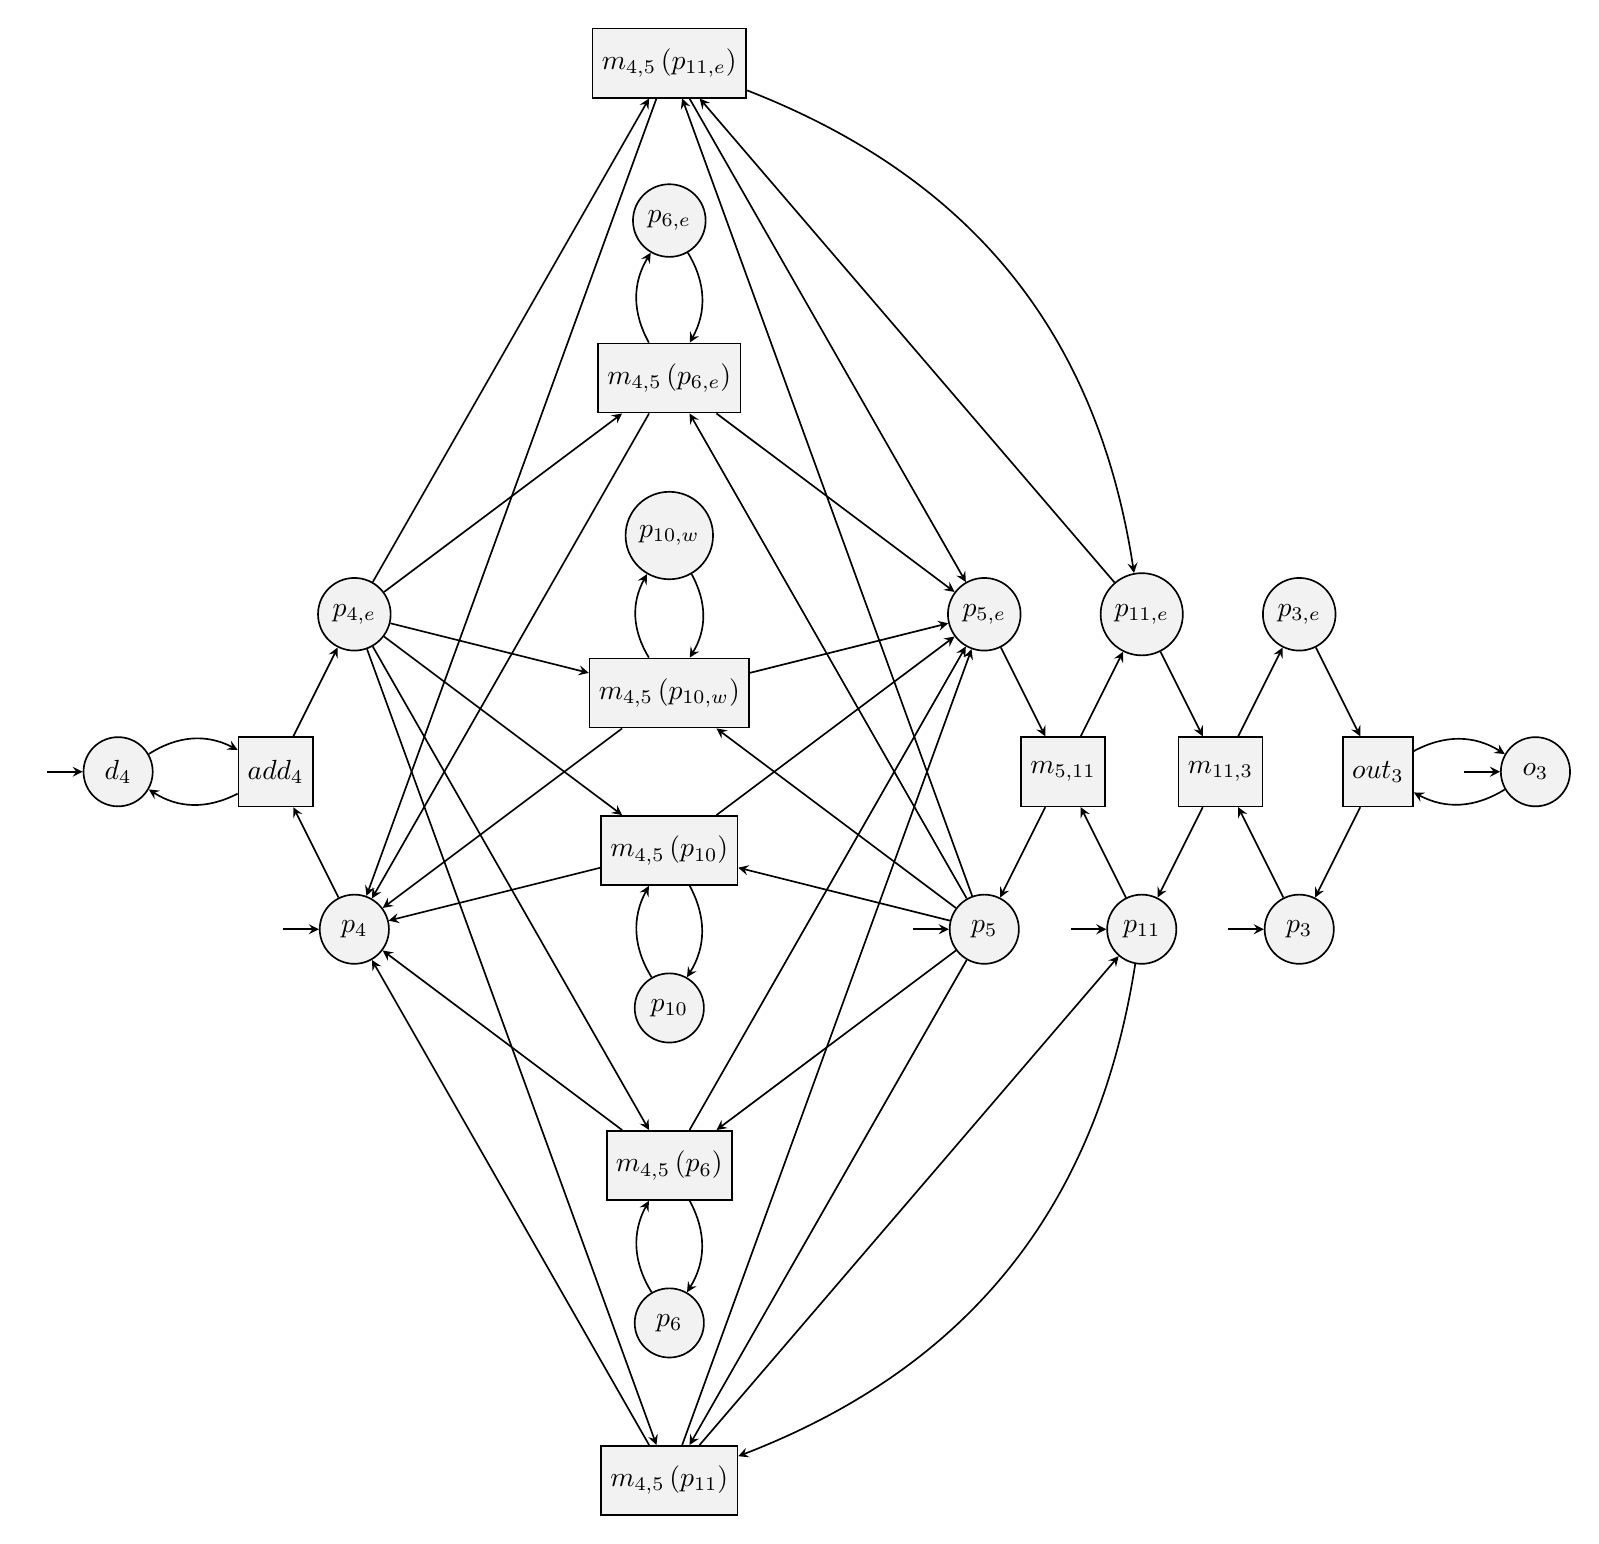
\begin{tikzpicture}
  \node[state, initial] at (0, 11) (d4){$d_4$};
  \node[state, initial] at (18, 11) (o3){$o_3$};

  \node[state, initial] at (3, 9) (p4){$p_4$};
  \node[state, initial] at (11, 9) (p5){$p_5$};
  \node[state, initial] at (13, 9) (p11){$p_{11}$};
  \node[state, initial] at (15, 9) (p3){$p_3$};

  \node[state] at (3, 13) (p4_e){$p_{4,e}$};
  \node[state] at (11, 13) (p5_e){$p_{5,e}$};
  \node[state] at (13, 13) (p11_e){$p_{11,e}$};
  \node[state] at (15, 13) (p3_e){$p_{3,e}$};

  \node[state, rectangle] at (2, 11) (add4){${add}_4$};
  \node[state, rectangle] at (12, 11) (m5_11){$m_{5,11}$};
  \node[state, rectangle] at (14, 11) (m11_3){$m_{11,3}$};
  \node[state, rectangle] at (16, 11) (out3){${out}_3$};

  \node[state] at (7, 4) (p6){$p_6$};
  \node[state] at (7, 8) (p10){$p_{10}$};
  \node[state] at (7, 18) (p6_e){$p_{6,e}$};
  \node[state] at (7, 14) (p10_w){$p_{10,w}$};

  \node[state, rectangle] at (7, 2) (m4_5__p11){$m_{4,5}\left(p_{11}\right)$};
  \node[state, rectangle] at (7, 6) (m4_5__p6){$m_{4,5}\left(p_6\right)$};
  \node[state, rectangle] at (7, 10) (m4_5__p10){$m_{4,5}\left(p_{10}\right)$};
  \node[state, rectangle] at (7, 20) (m4_5__p11_e){$m_{4,5}\left(p_{11,e}\right)$};
  \node[state, rectangle] at (7, 16) (m4_5__p6_e){$m_{4,5}\left(p_{6,e}\right)$};
  \node[state, rectangle] at (7, 12) (m4_5__p10_w){$m_{4,5}\left(p_{10,w}\right)$};

  \draw

  (d4) edge[bend left] (add4)
  (add4) edge[bend left] (d4)
  (p4) edge (add4)
  (add4) edge (p4_e)

  (p4_e) edge (m4_5__p11)
  (p4_e) edge (m4_5__p6)
  (p4_e) edge (m4_5__p10)
  (p4_e) edge (m4_5__p11_e)
  (p4_e) edge (m4_5__p6_e)
  (p4_e) edge (m4_5__p10_w)

  (m4_5__p11) edge (p4)
  (m4_5__p6) edge (p4)
  (m4_5__p10) edge (p4)
  (m4_5__p11_e) edge (p4)
  (m4_5__p6_e) edge (p4)
  (m4_5__p10_w) edge (p4)

  (p5) edge (m4_5__p11)
  (p5) edge (m4_5__p6)
  (p5) edge (m4_5__p10)
  (p5) edge (m4_5__p11_e)
  (p5) edge (m4_5__p6_e)
  (p5) edge (m4_5__p10_w)

  (m4_5__p11) edge (p5_e)
  (m4_5__p6) edge (p5_e)
  (m4_5__p10) edge (p5_e)
  (m4_5__p11_e) edge (p5_e)
  (m4_5__p6_e) edge (p5_e)
  (m4_5__p10_w) edge (p5_e)

  (p5_e) edge (m5_11)
  (m5_11) edge (p5)
  (p11) edge (m5_11)
  (m5_11) edge (p11_e)

  (p11_e) edge (m11_3)
  (m11_3) edge (p11)
  (p3) edge (m11_3)
  (m11_3) edge (p3_e)

  (p3_e) edge (out3)
  (out3) edge (p3)
  (o3) edge[bend left] (out3)
  (out3) edge[bend left] (o3)

  (p11) edge[bend left] (m4_5__p11)
  (m4_5__p11) edge (p11)
  (p11_e) edge (m4_5__p11_e)
  (m4_5__p11_e) edge[bend left] (p11_e)

  (p6) edge[bend left] (m4_5__p6)
  (m4_5__p6) edge[bend left] (p6)
  (p10) edge[bend left] (m4_5__p10)
  (m4_5__p10) edge[bend left] (p10)

  (p6_e) edge[bend left] (m4_5__p6_e)
  (m4_5__p6_e) edge[bend left] (p6_e)
  (p10_w) edge[bend left] (m4_5__p10_w)
  (m4_5__p10_w) edge[bend left] (p10_w)

  ;
\end{tikzpicture}

\subsection{$4 \rightarrow 10 \rightarrow 11 \rightarrow 3$}

The requirement here is still the same as the previous two routes as $5$, $6$, $10$ and $11$ is the place where deadlock could occur. A minor change is needed as now the route is driving towards $10$ instead of $5$ from $4$, but the graph is still similar

\begin{itemize}
  \item $\left\{ p_6 \rightarrow 1 \right\}$
  \item $\left\{ p_{6,e} \rightarrow 1 \right\}$
  \item $\left\{ p_{11} \rightarrow 1 \right\}$
  \item $\left\{ p_{11,e} \rightarrow 1 \right\}$
  \item $\left\{ p_{5} \rightarrow 1 \right\}$
  \item $\left\{ p_{5,w} \rightarrow 1 \right\}$
\end{itemize}

And the graph will then be

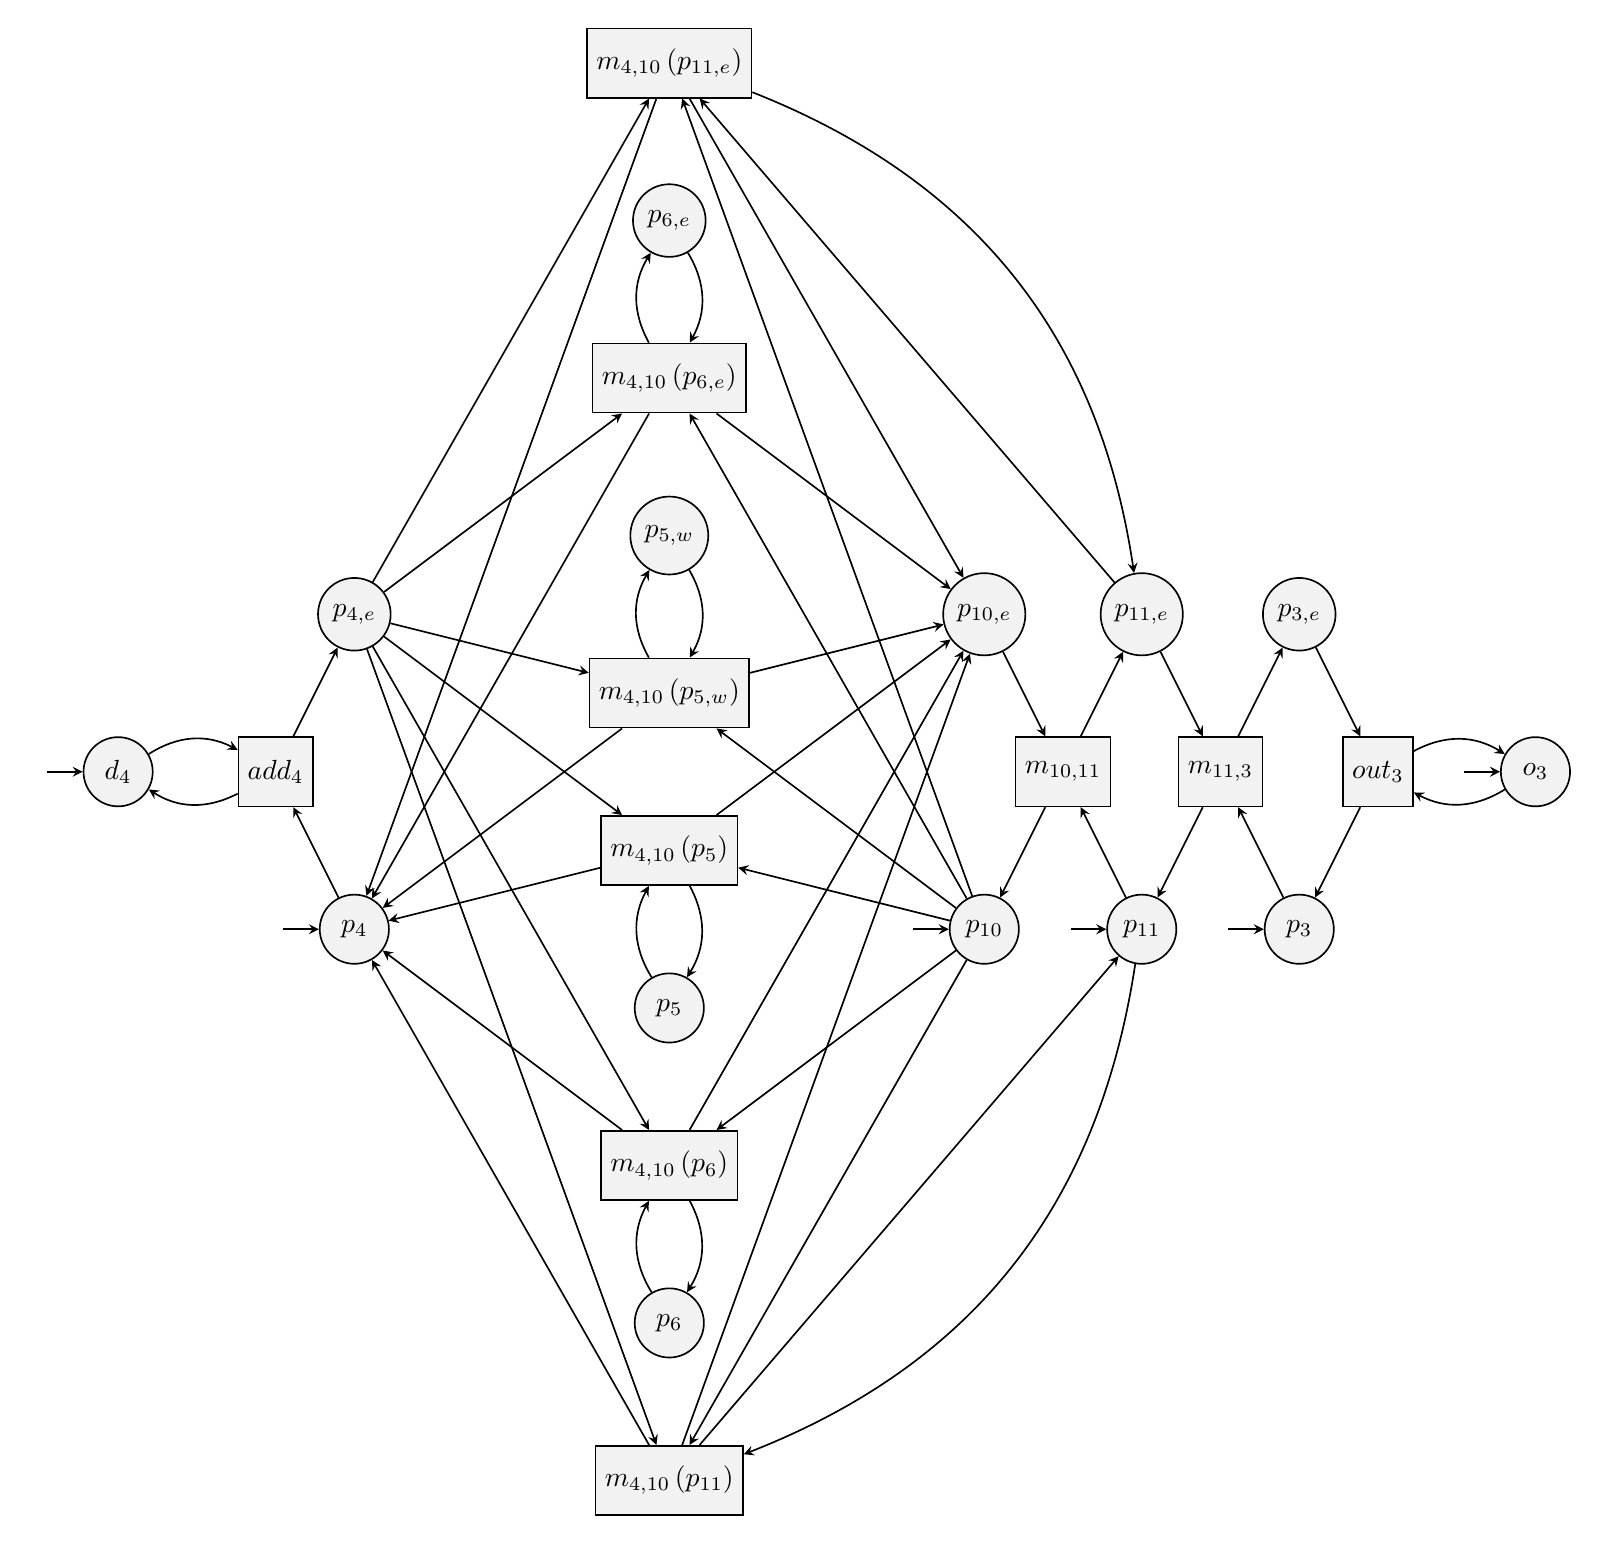
\begin{tikzpicture}
  \node[state, initial] at (0, 11) (d4){$d_4$};
  \node[state, initial] at (18, 11) (o3){$o_3$};

  \node[state, initial] at (3, 9) (p4){$p_4$};
  \node[state, initial] at (11, 9) (p10){$p_{10}$};
  \node[state, initial] at (13, 9) (p11){$p_{11}$};
  \node[state, initial] at (15, 9) (p3){$p_3$};

  \node[state] at (3, 13) (p4_e){$p_{4,e}$};
  \node[state] at (11, 13) (p10_e){$p_{10,e}$};
  \node[state] at (13, 13) (p11_e){$p_{11,e}$};
  \node[state] at (15, 13) (p3_e){$p_{3,e}$};

  \node[state, rectangle] at (2, 11) (add4){${add}_4$};
  \node[state, rectangle] at (12, 11) (m10_11){$m_{10,11}$};
  \node[state, rectangle] at (14, 11) (m11_3){$m_{11,3}$};
  \node[state, rectangle] at (16, 11) (out3){${out}_3$};

  \node[state] at (7, 4) (p6){$p_6$};
  \node[state] at (7, 8) (p5){$p_5$};
  \node[state] at (7, 18) (p6_e){$p_{6,e}$};
  \node[state] at (7, 14) (p5_w){$p_{5,w}$};

  \node[state, rectangle] at (7, 2) (m4_10__p11){$m_{4,10}\left(p_{11}\right)$};
  \node[state, rectangle] at (7, 6) (m4_10__p6){$m_{4,10}\left(p_6\right)$};
  \node[state, rectangle] at (7, 10) (m4_10__p5){$m_{4,10}\left(p_5\right)$};
  \node[state, rectangle] at (7, 20) (m4_10__p11_e){$m_{4,10}\left(p_{11,e}\right)$};
  \node[state, rectangle] at (7, 16) (m4_10__p6_e){$m_{4,10}\left(p_{6,e}\right)$};
  \node[state, rectangle] at (7, 12) (m4_10__p5_w){$m_{4,10}\left(p_{5,w}\right)$};

  \draw

  (d4) edge[bend left] (add4)
  (add4) edge[bend left] (d4)
  (p4) edge (add4)
  (add4) edge (p4_e)

  (p4_e) edge (m4_10__p11)
  (p4_e) edge (m4_10__p6)
  (p4_e) edge (m4_10__p5)
  (p4_e) edge (m4_10__p11_e)
  (p4_e) edge (m4_10__p6_e)
  (p4_e) edge (m4_10__p5_w)

  (m4_10__p11) edge (p4)
  (m4_10__p6) edge (p4)
  (m4_10__p5) edge (p4)
  (m4_10__p11_e) edge (p4)
  (m4_10__p6_e) edge (p4)
  (m4_10__p5_w) edge (p4)

  (p10) edge (m4_10__p11)
  (p10) edge (m4_10__p6)
  (p10) edge (m4_10__p5)
  (p10) edge (m4_10__p11_e)
  (p10) edge (m4_10__p6_e)
  (p10) edge (m4_10__p5_w)

  (m4_10__p11) edge (p10_e)
  (m4_10__p6) edge (p10_e)
  (m4_10__p5) edge (p10_e)
  (m4_10__p11_e) edge (p10_e)
  (m4_10__p6_e) edge (p10_e)
  (m4_10__p5_w) edge (p10_e)

  (p10_e) edge (m10_11)
  (m10_11) edge (p10)
  (p11) edge (m10_11)
  (m10_11) edge (p11_e)

  (p11_e) edge (m11_3)
  (m11_3) edge (p11)
  (p3) edge (m11_3)
  (m11_3) edge (p3_e)

  (p3_e) edge (out3)
  (out3) edge (p3)
  (o3) edge[bend left] (out3)
  (out3) edge[bend left] (o3)

  (p11) edge[bend left] (m4_10__p11)
  (m4_10__p11) edge (p11)
  (p11_e) edge (m4_10__p11_e)
  (m4_10__p11_e) edge[bend left] (p11_e)

  (p6) edge[bend left] (m4_10__p6)
  (m4_10__p6) edge[bend left] (p6)
  (p5) edge[bend left] (m4_10__p5)
  (m4_10__p5) edge[bend left] (p5)

  (p6_e) edge[bend left] (m4_10__p6_e)
  (m4_10__p6_e) edge[bend left] (p6_e)
  (p5_w) edge[bend left] (m4_10__p5_w)
  (m4_10__p5_w) edge[bend left] (p5_w)

  ;
\end{tikzpicture}

\section{Entering from $8$}

As this is the reverse route, we can start from the bottom to avoid potential collision first.

\subsection{$8 \rightarrow 12 \rightarrow 13 \rightarrow 10 \rightarrow 9$}

This is the simplest route as this is not part of the potential deadlock. When the train drives to $10$, it can safely exit via $9$. The graph is

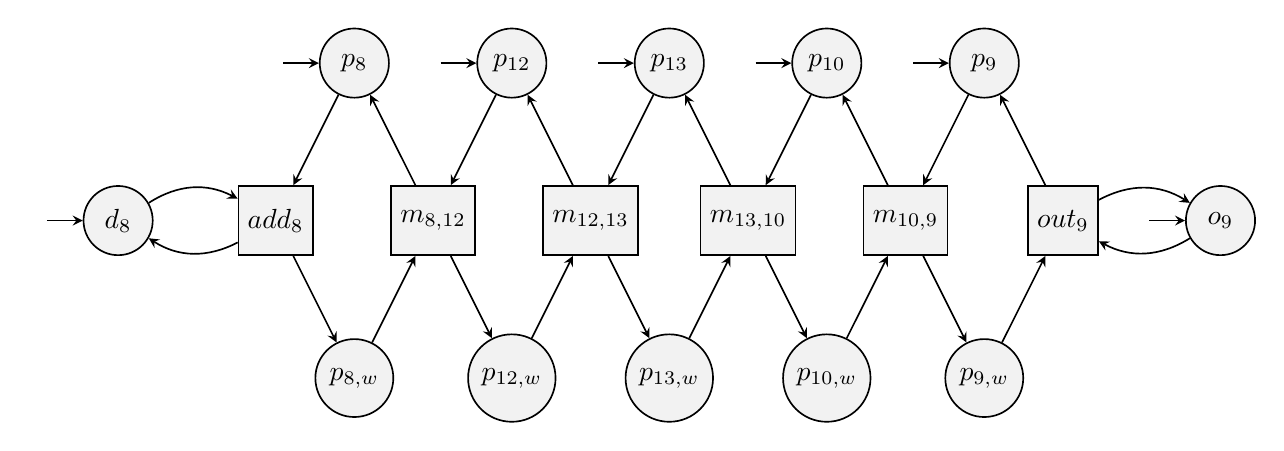
\begin{tikzpicture}
  \node[state, initial] at (0, 2) (d8){$d_8$};
  \node[state, initial] at (14, 2) (o9){$o_9$};

  \node[state, initial] at (3, 4) (p8){$p_8$};
  \node[state, initial] at (5, 4) (p12){$p_{12}$};
  \node[state, initial] at (7, 4) (p13){$p_{13}$};
  \node[state, initial] at (9, 4) (p10){$p_{10}$};
  \node[state, initial] at (11, 4) (p9){$p_9$};

  \node[state] at (3, 0) (p8_w){$p_{8,w}$};
  \node[state] at (5, 0) (p12_w){$p_{12,w}$};
  \node[state] at (7, 0) (p13_w){$p_{13,w}$};
  \node[state] at (9, 0) (p10_w){$p_{10,w}$};
  \node[state] at (11, 0) (p9_w){$p_{9,w}$};

  \node[state, rectangle] at (2, 2) (add8){${add}_8$};
  \node[state, rectangle] at (4, 2) (m8_12){$m_{8,12}$};
  \node[state, rectangle] at (6, 2) (m12_13){$m_{12,13}$};
  \node[state, rectangle] at (8, 2) (m13_10){$m_{13,10}$};
  \node[state, rectangle] at (10, 2) (m10_9){$m_{10,9}$};
  \node[state, rectangle] at (12, 2) (out9){${out}_9$};

  \draw

  (d8) edge[bend left] (add8)
  (add8) edge[bend left] (d8)
  (p8) edge (add8)
  (add8) edge (p8_w)

  (p8_w) edge (m8_12)
  (m8_12) edge (p8)
  (p12) edge (m8_12)
  (m8_12) edge (p12_w)

  (p12_w) edge (m12_13)
  (m12_13) edge (p12)
  (p13) edge (m12_13)
  (m12_13) edge (p13_w)

  (p13_w) edge (m13_10)
  (m13_10) edge (p13)
  (p10) edge (m13_10)
  (m13_10) edge (p10_w)

  (p10_w) edge (m10_9)
  (m10_9) edge (p10)
  (p9) edge (m10_9)
  (m10_9) edge (p9_w)

  (p9_w) edge (out9)
  (out9) edge (p9)
  (o9) edge[bend left] (out9)
  (out9) edge[bend left] (o9)

  ;
\end{tikzpicture}

\section{Priority}

Despite the design above, it's important to introduce the concept of priority to prioritise the selection of track in each intersection. This can avoid blocking one of the train entrance permanently when the system is busy. This is especially important to the outgoing track from $3$ as trains entering from $1$ and $4$ will merge into track $3$.

\end{document}
